% Chapter Template

\chapter{Results} % Main chapter title

\label{sec:results} % Change X to a consecutive number; for referencing this chapter elsewhere, use \ref{ChapterX}

\lhead{\emph{Results}} % Change X to a consecutive number; this is for the header on each page - perhaps a shortened title

%----------------------------------------------------------------------------------------
%	SECTION 1
%----------------------------------------------------------------------------------------
The main results of this thesis are summarized in Fig.
\ref{fig:CentralSpec} and \ref{fig:HomSpec}.
They show 2D histograms of the escape frequency $x$ and outgoing angle
$\theta$ parametrized by $|\mu|$.
Taking into account only photons photons around a value
of $|\mu|$ gives us the emission detected by an observer located at an
angle $\theta$ with respect to the rotation axis.
We have verified that the solutions are indeed symmetric with respect
to $\mu=0$. We have also verified that the total flux is the same for all $\mu$.
From these figures we can see that the line properties change with
rotational velocity and depend on the viewing angle $\theta$.
In the next subsections we quantify the morphology changes with with
velocity, optical depth and viewing angle.
We characterize the line morphology by its total intensity, the full
width at half maximum, (FWHM) and the location of the peak maxima.
In order to interpret the
morphological changes in the line we also report the median number of
scatter for each \ly photon in the simulation.
For the models where dust is included we measure the escape fraction
as a function of rotational velocity and viewing angle.
\subsection{Line Morphology}
\label{sec:angles}
The first column in both Fig. \ref{fig:CentralSpec} and
\ref{fig:HomSpec} shows that for the static sphere the line properties
are independent of $|\mu|$, as it is expected due
to the spherical symmetry.
However, for increasing rotational velocities, at a fixed optical
depth, there are clear signs that this symmetry is broken.
If the viewing angle is aligned with the rotation axis, $|\mu|\sim
1$, the \ly line keeps a double peak with minor
changes in the morphology as the rotational velocity increases.
However, for a line of sight perpendicular to the rotation axis,
$|\mu|\sim 0$, the impact of rotation is larger.
The double peak readily transforms into a single peak.
This is clear in Fig. \ref{fig:differentvelocities} and in Fig.
\ref{fig:differentvelocities2} where we
present the different line morphologies for $|\mu|\sim 0$ and
$|\mu|\sim 1 $ for the
homogeneous and central configurations.
The panels have the same distribution as Fig. \ref{fig:CentralSpec}
and \ref{fig:HomSpec}.
There are three clear effects on the line morphology as the rotational
velocity increases.
First, the line broadens; second, the double peaks reduce their intensity; and
third, the intensity at the line centre rises.
The last two effects are combined to give the impression that the double
peaks are merged into a single one at high rotational velocities.
\subsection{Integrated Line Intensity}
\label{sec:intlineint}
\begin{figure}
\begin{center}
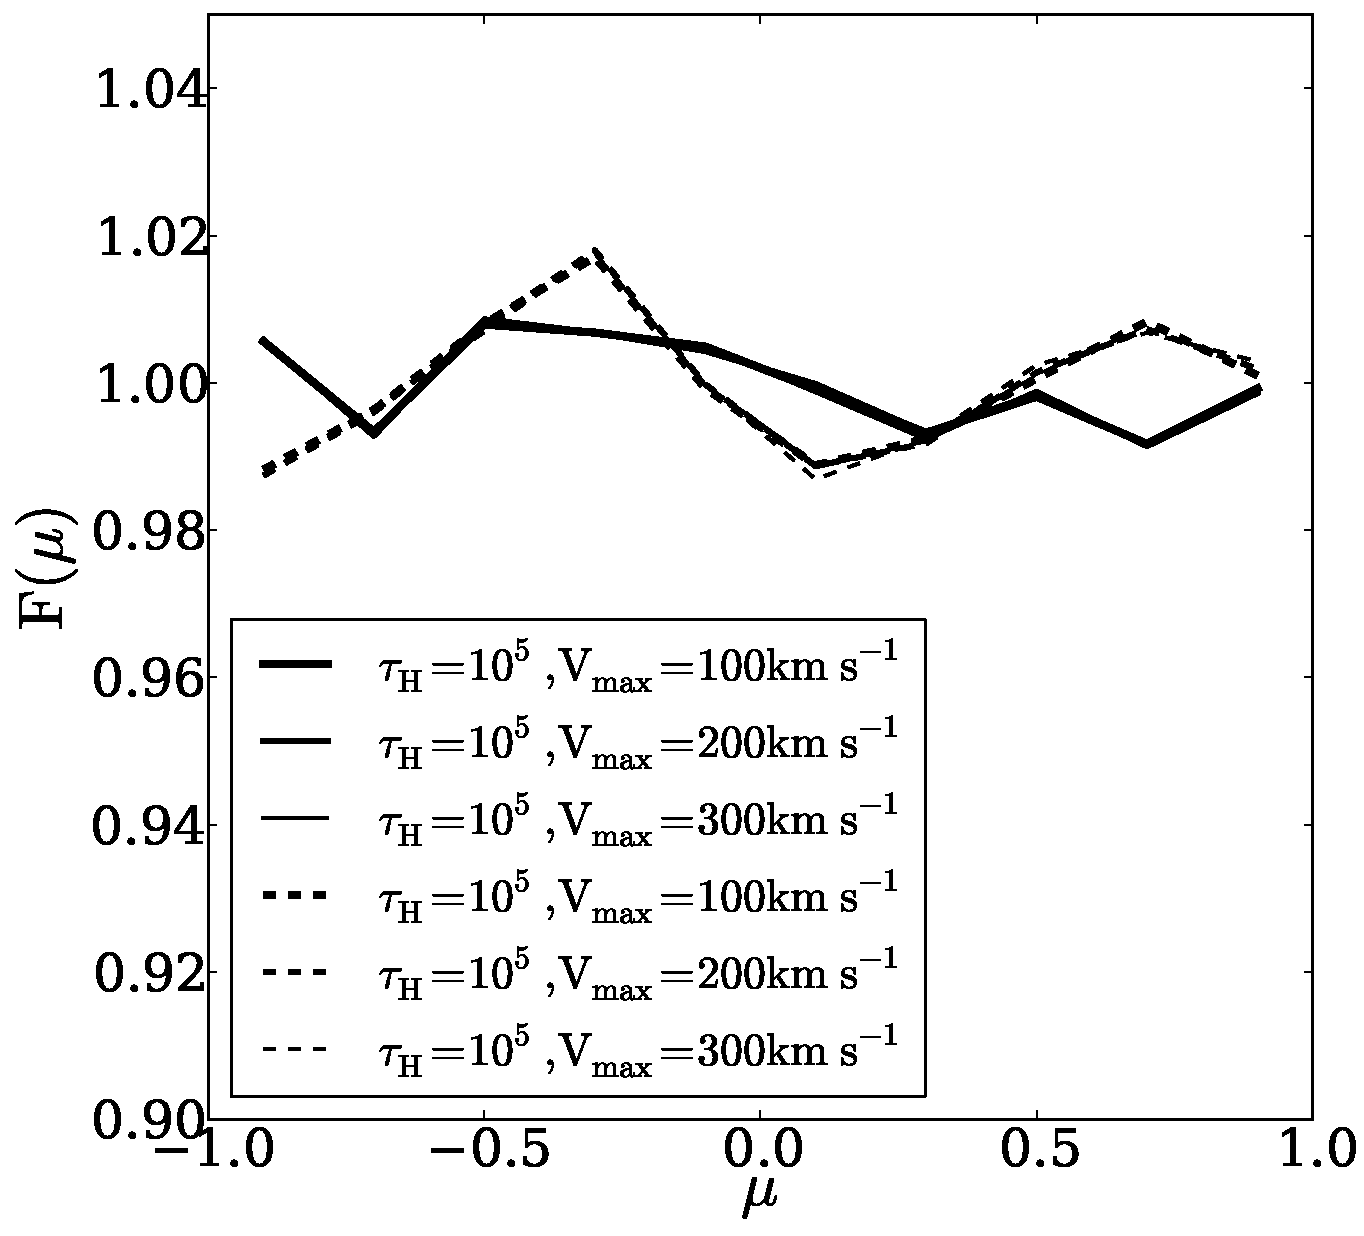
\includegraphics[width=0.4\textwidth]{../Figures/f5.pdf}
\end{center}
\caption{Integrated flux distribution as a function of the
viewing angle as parametrized by $\mu$. Continuous (dashed)
correspond to central (homogeneous) source distribution.
The models correspond to an optical depth of $\tau_{\rm
H}=10^5$ and rotational velocities of $100$\kms, $200$\kms and
$300$\kms. The distributions are flat in the range of models probed
in this work, meaning that the integrated flux for all viewing
angles is the same.
\label{fig:muhisto}}
\end{figure}
We now consider possible variations in the integrated flux with
respect to the viewing angle $\theta$.
To this end we define the normalized flux seen by an observer at an
angle $\mu$ by:
\begin{equation}
F(\mu) = \frac{2\Delta N}{N\Delta \mu},
\end{equation}
%
where $\mu=\cos\theta$, $N$ is the total number of outgoing photons,
$\Delta N$ is the number of photons in an angular bin $\Delta
\theta$. This definition satisfies the condition
$\int_{-1}^{1}F(\mu)d\mu/2=1$. In the case of perfect spherical
symmetry one expects a flat distribution with $F(\mu)=1$.
Fig. \ref{fig:muhisto} shows the results for a selection of models
with $\tau_{\rm H}=10^{5}$, different rotational velocities and the two
types of source distributions. This shows that $F(\mu)$ is consistent with being flat, apart
from some statistical fluctuations on the order of 2\%.
This is a remarkable result: while the rotation axis defines preferential direction, the
integrated flux is the same for all viewing angles in the range of parameters explored in this paper. This can be understood from the fact that
{\it radiative transfer inside a sphere that undergoes solid-body
rotation proceeds identical as inside a static sphere}: we can draw
a line between any two atoms within the rotating cloud, and their
relative velocity along this line is zero (apart from the relative
velocity as a result of random thermal motion), irrespective of the
rotation velocity of the cloud. This relative velocity is what is
relevant for the radiative transfer\footnote{This point can be further
illustrated by considering the path of individual photons: let a
photon be emitted at line center ($x=0$), in some random direction
${\bf k}$, propagate a distance that corresponds to $\tau_0=1$,
scatter fully coherently (i.e. $x=0$ after scattering in the gas
frame) by 90$^{\circ}$, and again propagate a distance that
corresponds to $\tau_0=1$. The position where the photon scatters
next does {\it not} depend on the rotation of the cloud, nor on
${\bf k}$.}
\subsection{Full Width at Half Maximum}
\label{sec:widthpeak}
\begin{figure*}
\begin{center}
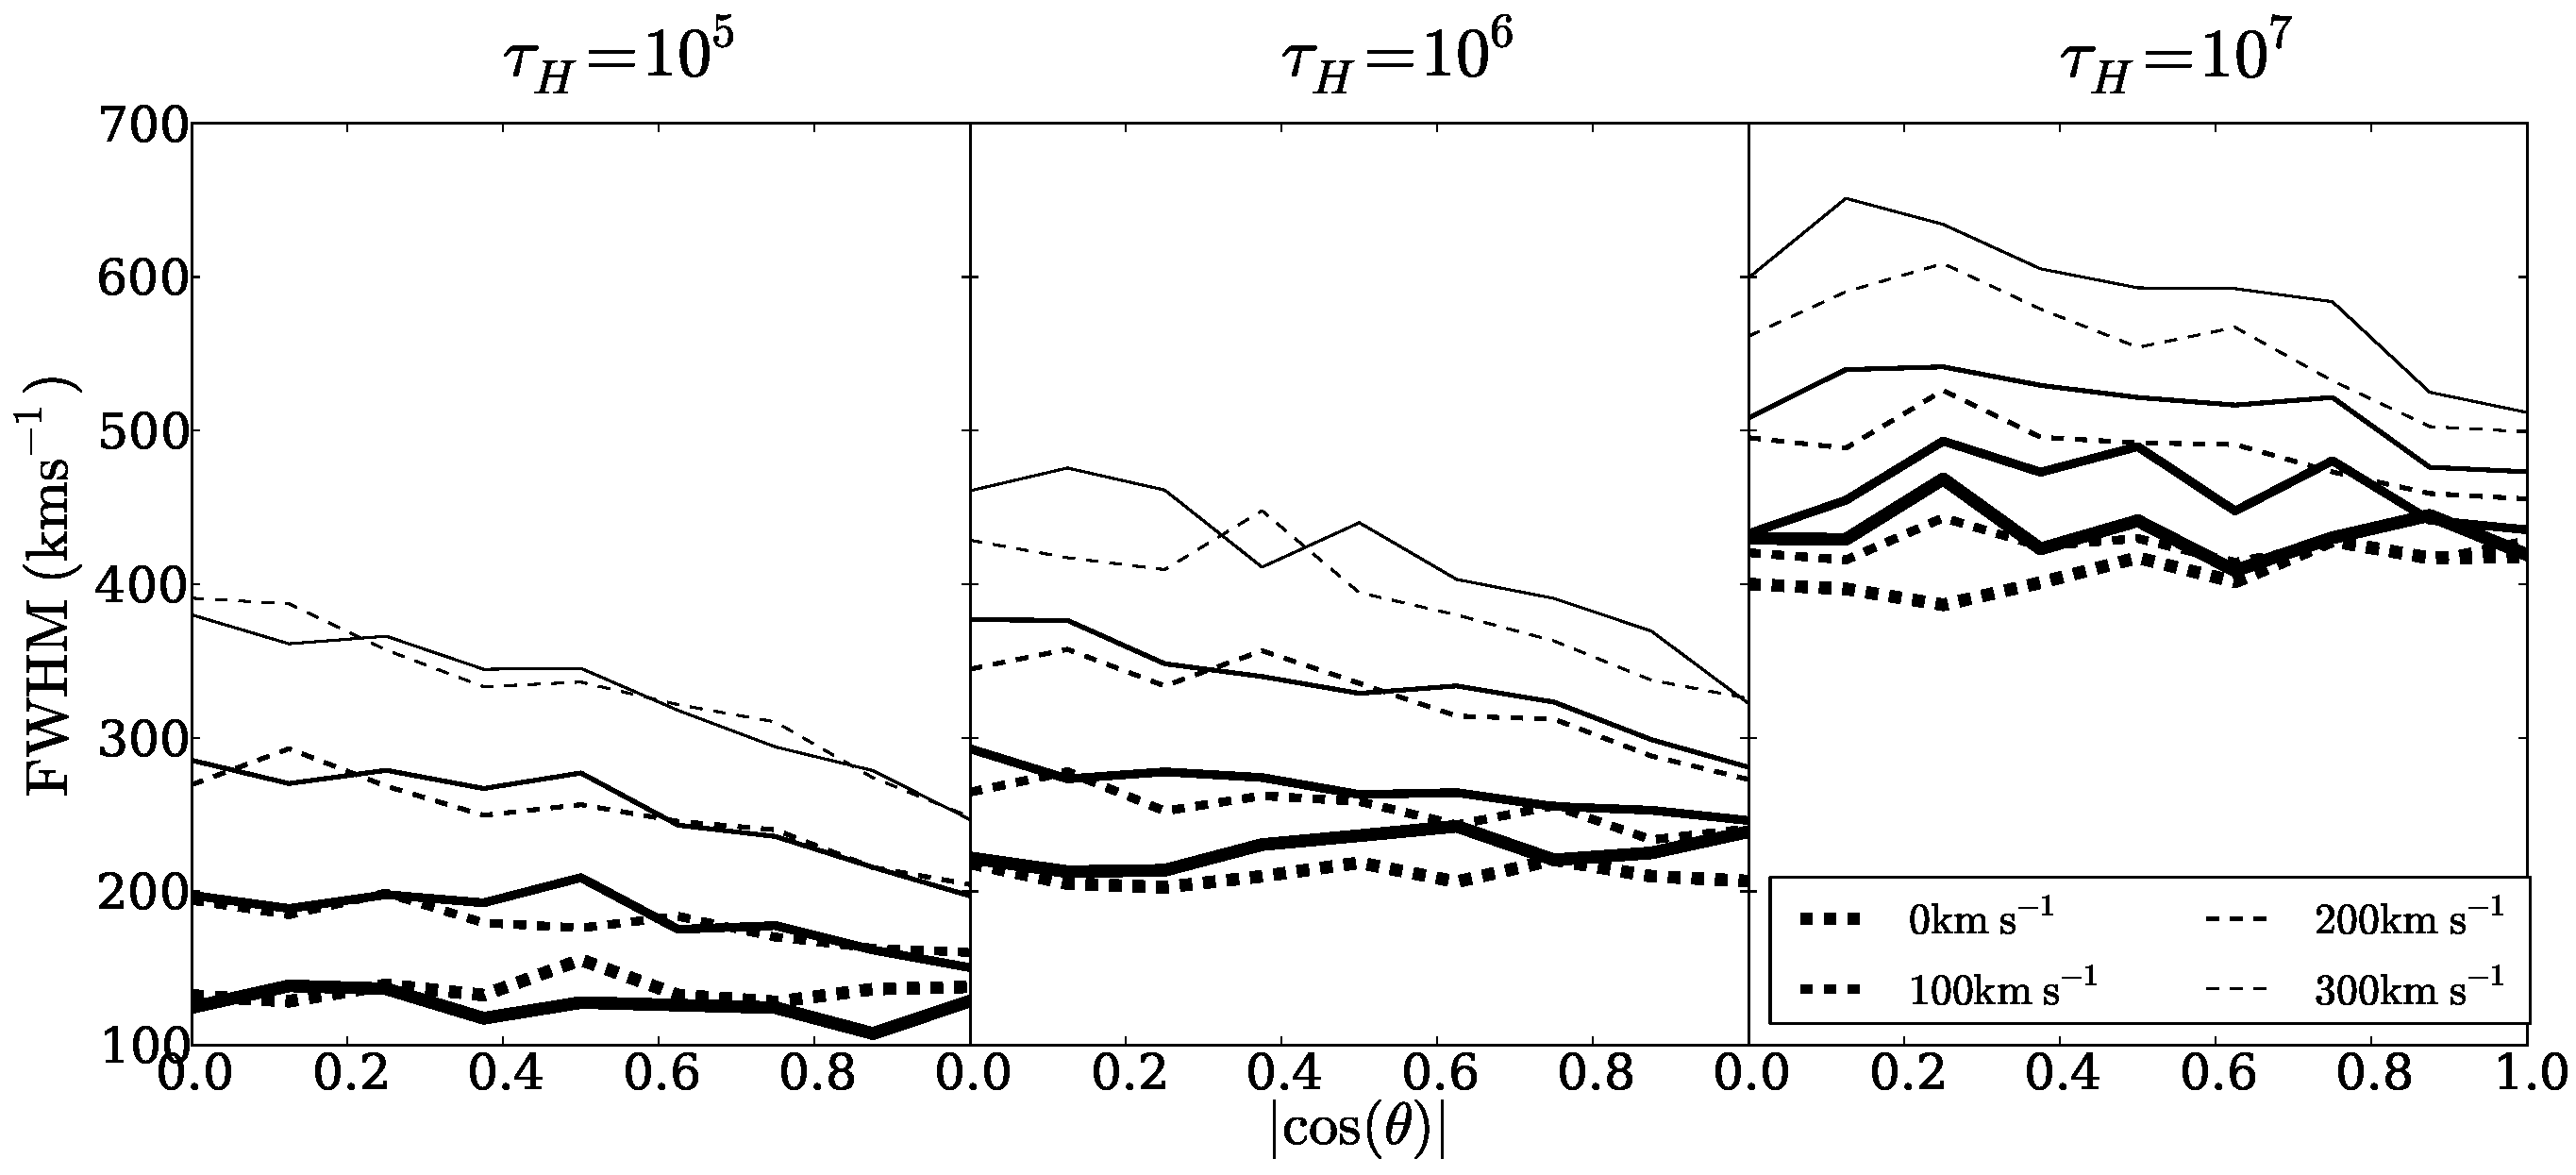
\includegraphics[width=0.95\textwidth]{../Figures/f6.pdf}
\end{center}
\caption{FWHM for the non-dusty models as a function of the viewing
angle parametrized by $|\cos\theta|$. Continuous (dashed) lines correspond
to central (homogeneous) source distributions. The general trend is
of an decreasing line width as the line of sight becomes parallel to the
rotation axis.
\label{fig:widthvsmu}}
\end{figure*}
\begin{figure*}
\begin{center}
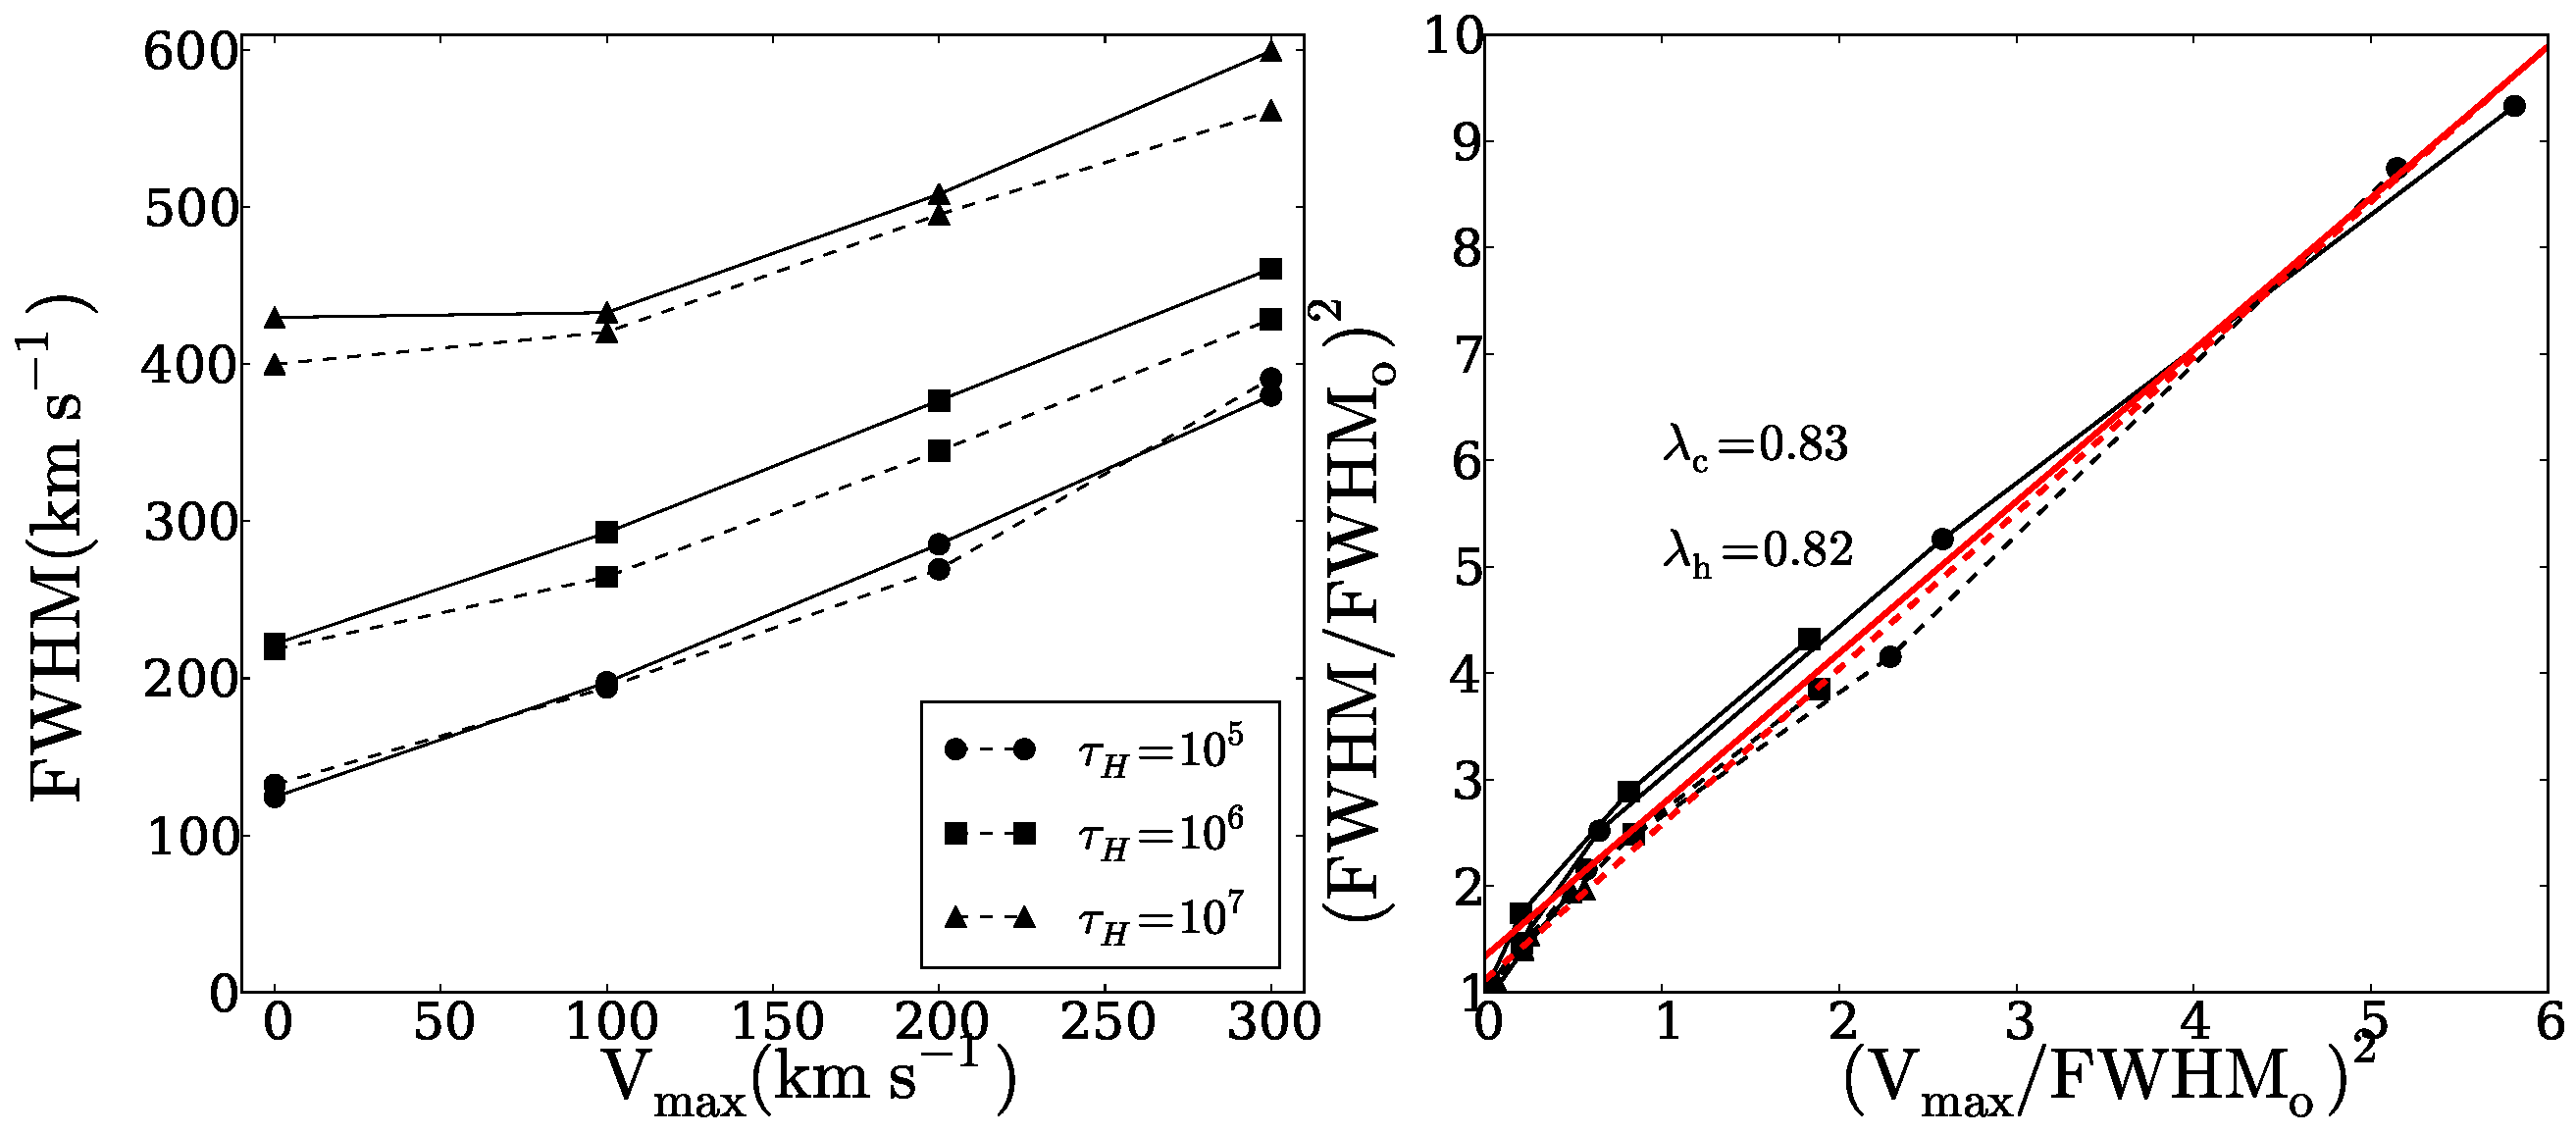
\includegraphics[width=0.95\textwidth]{../Figures/f7.pdf}
\end{center}
\caption{FWHM for the non-dusty models as a function of
rotational velocity $V_{\rm max}$ for observers located
perpendicular to the rotation axis.
The left panel shows the results in velocity units while the right
panel normalizes the data by the FWHM in the static case.
Continuous (dashed) lines correspond to central (homogeneous)
source distributions.
The straight lines represent the fit to the data using the
expression in Eq. (\ref{eq:fwhm}).
\label{fig:widthsvsvelocity}}
\end{figure*}
We use the full width at half maximum (FWHM) to quantify the line
broadening.
We measure this width from the line intensity histogram by finding the
values of the velocities at half maximum intensity.
We use lineal interpolation between histogram points to get a value
more precise than the bin size used to construct the histogram.
Fig. \ref{fig:widthvsmu} shows the FWHM for all models as a function
of the viewing angle.
The FWHM increases for decreasing values of $\mu$ (movement from the
poles to the equator) and increasing values of $V_{\rm max}$.
In Fig.
\ref{fig:widthsvsvelocity} we fix $|\mu|<0.1$, i.e. viewing angle
perpendicular to the rotation axis, to plot the FWHM as a function of
rotational velocity.
We parametrize the dependency of the line width with $V_{\rm max}$ as
%
\begin{equation}
{\rm FWHM}^2 = {\rm FWHM}_{0}^2 + V_{\rm max}^2/\lambda^2,
\label{eq:fwhm}
\end{equation}
%
where FWHM$_{0}$ is the velocity width in the static case and $\lambda$
is a positive scalar to be determined as a fit to the data.
With this test we want to know to what extent the new velocity width can be
expressed as a quadratic sum of the two relevant velocities in the
problem.
All the models fall into a single family of lines in the plane shown
in the right panel of Fig. \ref{fig:widthsvsvelocity}, justifying
the choice of our parametrization.
We fit simultaneously all the points in two separate groups, central
and homogeneous sources.
We find that these values are $\lambda_{\rm c} = 0.83 \pm 0.06$ and
$\lambda_{\rm h}= 0.82\pm 0.05$ respectively.
\subsection{Line Maxima}
\label{sec:maxima}
\begin{figure*}
\begin{center}
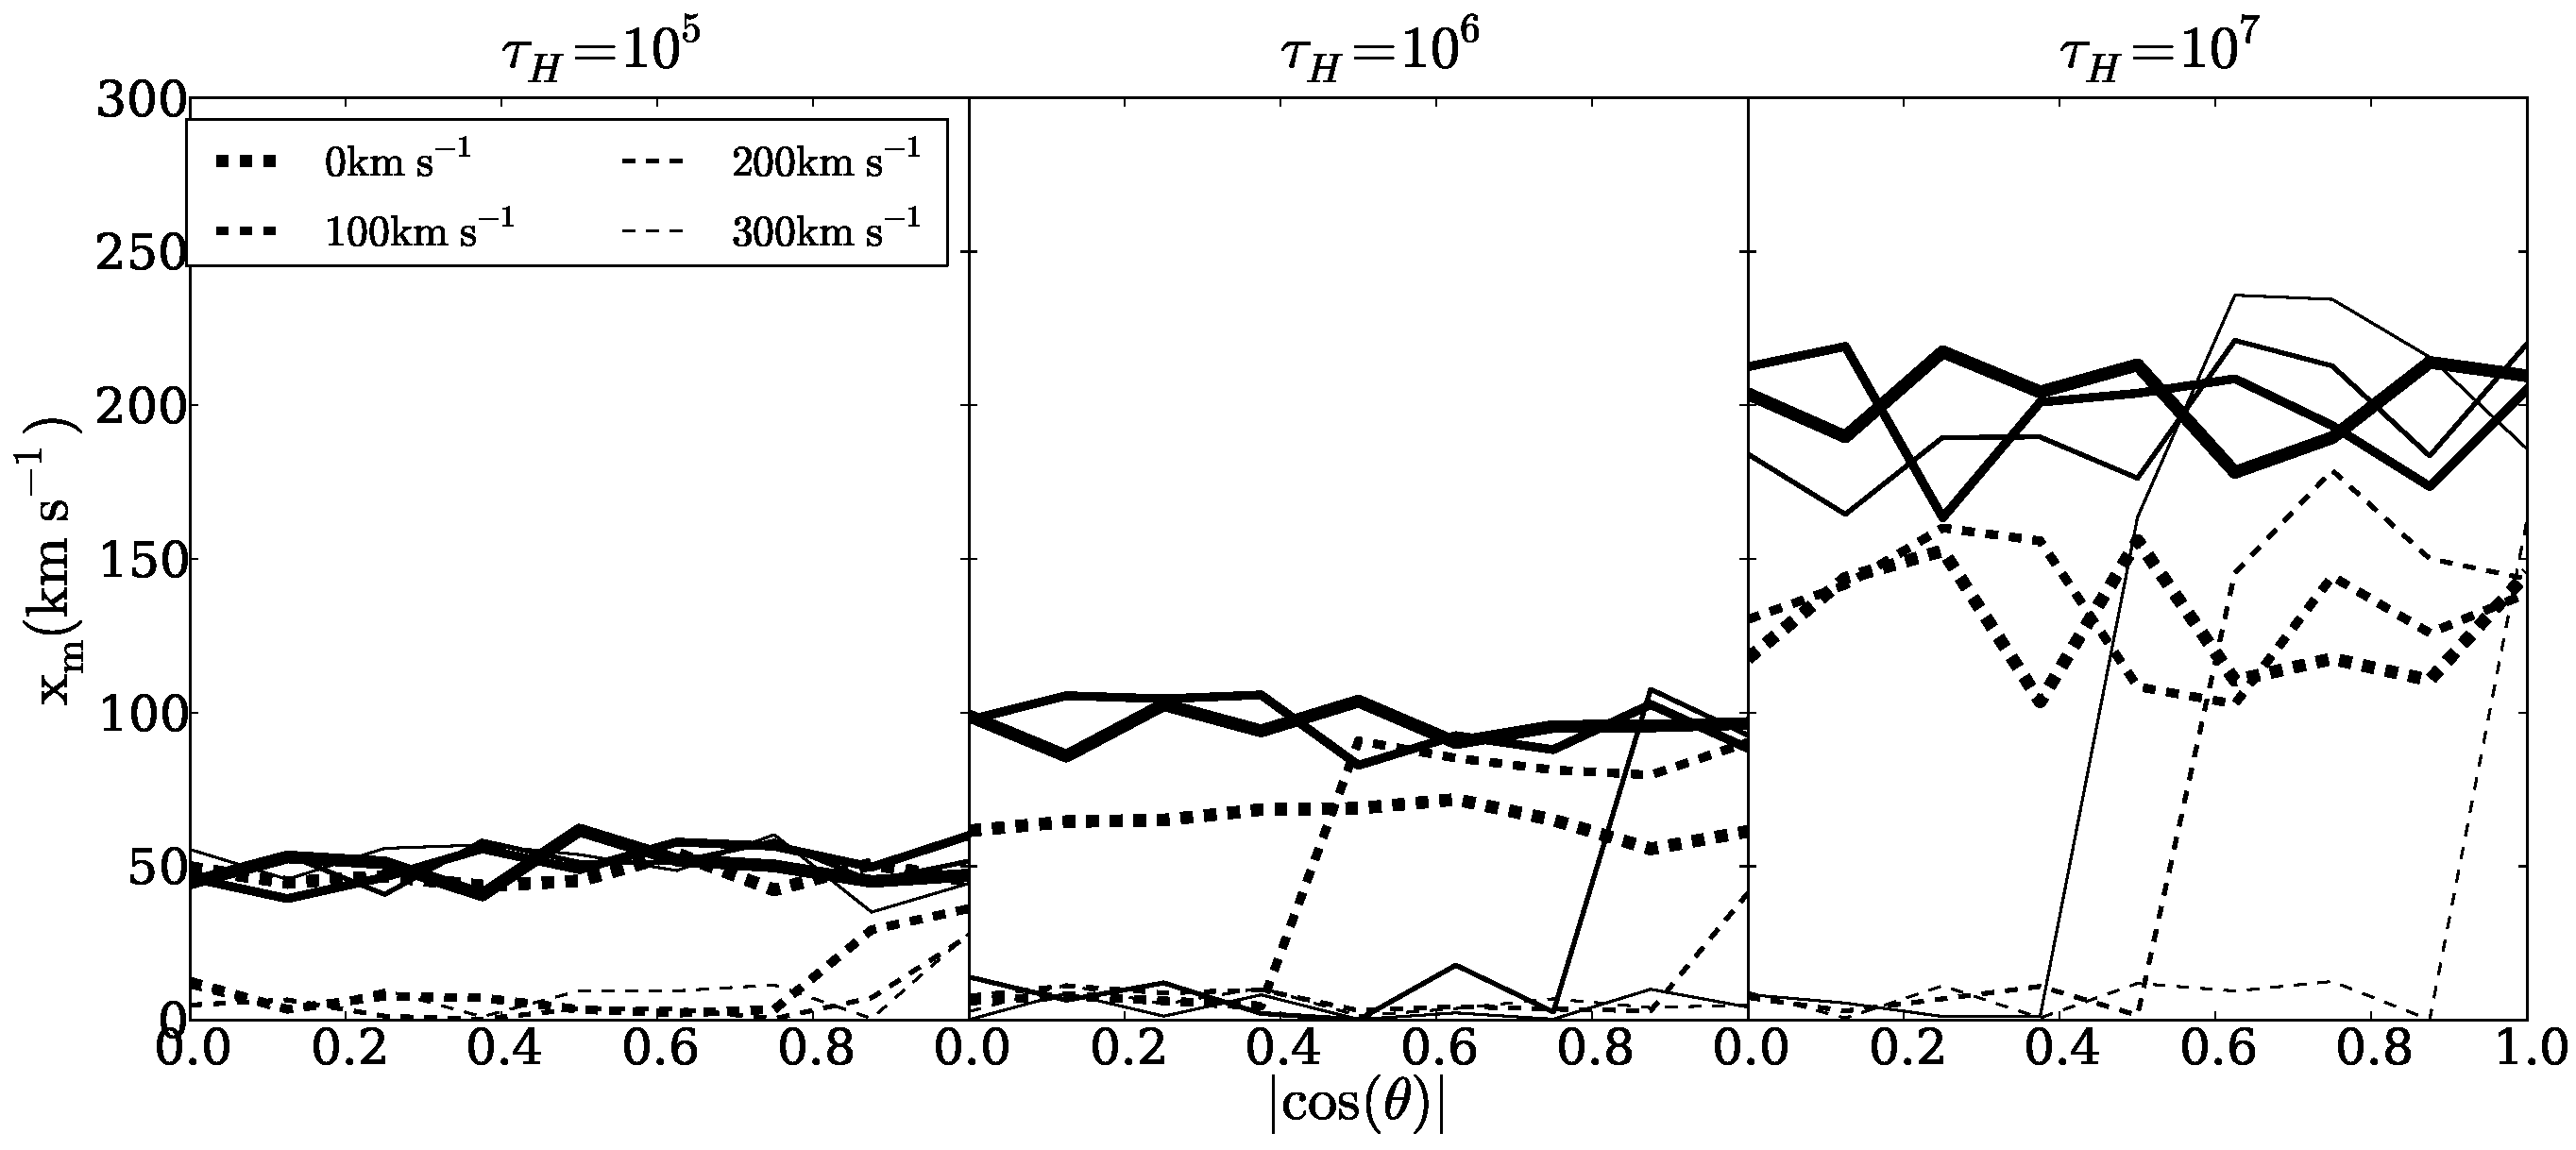
\includegraphics[width=0.95\textwidth]{../Figures/f8.pdf}
\end{center}
\caption{Position of the line maxima as a function of maximum
rotational velocity $V_{\rm max}$. Continuous (dashed) lines
correspond to central (homogeneous) source distributions. A value
of $x_{\rm max}=0$ indicates that line becomes single
peaked. \label{fig:maximumvsvelocity}}
\end{figure*}
We measure the peak maxima position, $x_m$, to quantify the transition from
double into single peak profiles.
In Fig. \ref{fig:maximumvsvelocity} we show the dependence of $x_m$ with
the viewing angle parametrized by $|\cos\theta|$ for different
rotational velocities.
There are two interesting features that deserve attention.
First, for a viewing angle parallel to the rotational axis ($\mu\sim
1.0$) the maxima of all models with the same kind of source
initialization are similar regardless of the rotational velocity.
Second, at a viewing angle perpendicular to the rotation axis ($\mu\sim 0.0$) a
large fraction of models become single peaked.
This feature appears more frequently for homogeneously distributed
sources if all the other parameters are equal.
\subsection{Dusty Clouds: Escape Fraction}
\label{sec:escapefraction}
\begin{table}
\begin{center}
\begin{tabular}{c cccccc}
\hline \hline
Source & $\tau_{H}$ & & $\ V_{\rm max}$& & \\
Distribution& & & (\kms) & & \\
& & 0 & 100 &200 & 300\\ \hline
Homogeneous & $10^{5}$& 0.263 & 0.263 & 0.263 & 0.263 \\
& $10^{6}$ & 0.291 & 0.292 & 0.293 & 0.293 \\
&$10^{7}$ & 0.228 & 0.228 & 0.228 & 0.228 \\
Central & $10^{5}$ & 0.096 & 0.096 & 0.096 & 0.096 \\
&$10^{6}$ & 0.066 & 0.066 & 0.066 & 0.066 \\
&$10^{7}$ & 0.015 & 0.016 & 0.016 & 0.015 \\
\hline
\end{tabular}
\caption{
Escape fraction values for all dusty models. }
\label{table:escape}
\end{center}
\end{table}
We now estimate the escape fraction $f_{\rm esc}$ for the dusty
models. The main result is that we do not find any significant dependence
with either the viewing angle nor the rotational velocity. This is consistent with our finding in \S~\ref{sec:intlineint}, that radiative transfer inside the cloud does not depend on its rotational velocity. For completeness we list in Table \ref{table:escape} the escape
fraction for all models.
We now put these results in the context of the analytic solution for
the infinite slab\citep{Neufeld90}.
In Neufeld's set-up the analytic solution depends
uniquely on the product $(a\tau_{\rm H})^{1/3}\tau_{A}$ where
$\tau_{A} = (1 - A)\tau_{a}$, valid only in the limit $a\tau_{\rm
H}\gg 1$.
At fixed values of $\tau_{a}$ the escape fraction monotonically
decreases with increasing values of $\tau_{\rm H}$.
This expectation holds for the central sources.
But in the case of homogeneous sources the escape fraction increases
slightly from $\tau_{\rm H}=10^5$ to $\tau_{\rm H}=10^{6}$
The naive interpretation of the analytic solution does not seem to
hold for photons emitted far from the sphere's center.
We suggest that increasing $\tau_{\rm H}$ from $10^{5}$ to $10^{6}$ causes a
transition from the 'optically thick' to the 'extremely optically
thick' regime for a noticeable fraction of the photons in the
homogeneous source distribution.
In the optically thick regime, \ly photons can escape in
'single flight' which corresponds to a scenario in which the
photon resonantly scatters $10^4-10^5$ times until it is scattered
into the wing of the line ($x\sim 3-4$).
At these frequencies the medium is optically thin, and the photons can
escape efficiently in a single flight.
In contrast, in an extremely optically thick medium \ly
photons escape in a `single excursion' \citep{Adams72}.
Here, photons that are scattered into the wing of the line escape from
the medium in a sequence of wing scattering events.
In both cases, \ly photons resonantly scatter $10^4$-$10^5$ times.
Because we keep our clouds the same size, the mean free path of Lya
photons that scatter resonantly is 10 times larger for the case
$\tau_{\rm H}=10^5$ than for $\tau_{\rm H}=10^6$.
If we compute the average distance $D$ travelled by \ly
photons through a medium of size $R$ as a function of line center
optical depth $\tau_{\rm H}$, then we find that during the transition
from optically thick to extremely optically thick the mean traversed
distance $D$ actually decreases slightly.
This decrease is unique to this transition region, and $D$ generally
increases with $\tau_{\rm H}$ at other values of $\tau_{\rm H}$.
\subsection{Average Number of Scatterings}
\label{sec:scatterings}
\begin{figure*}
\begin{center}
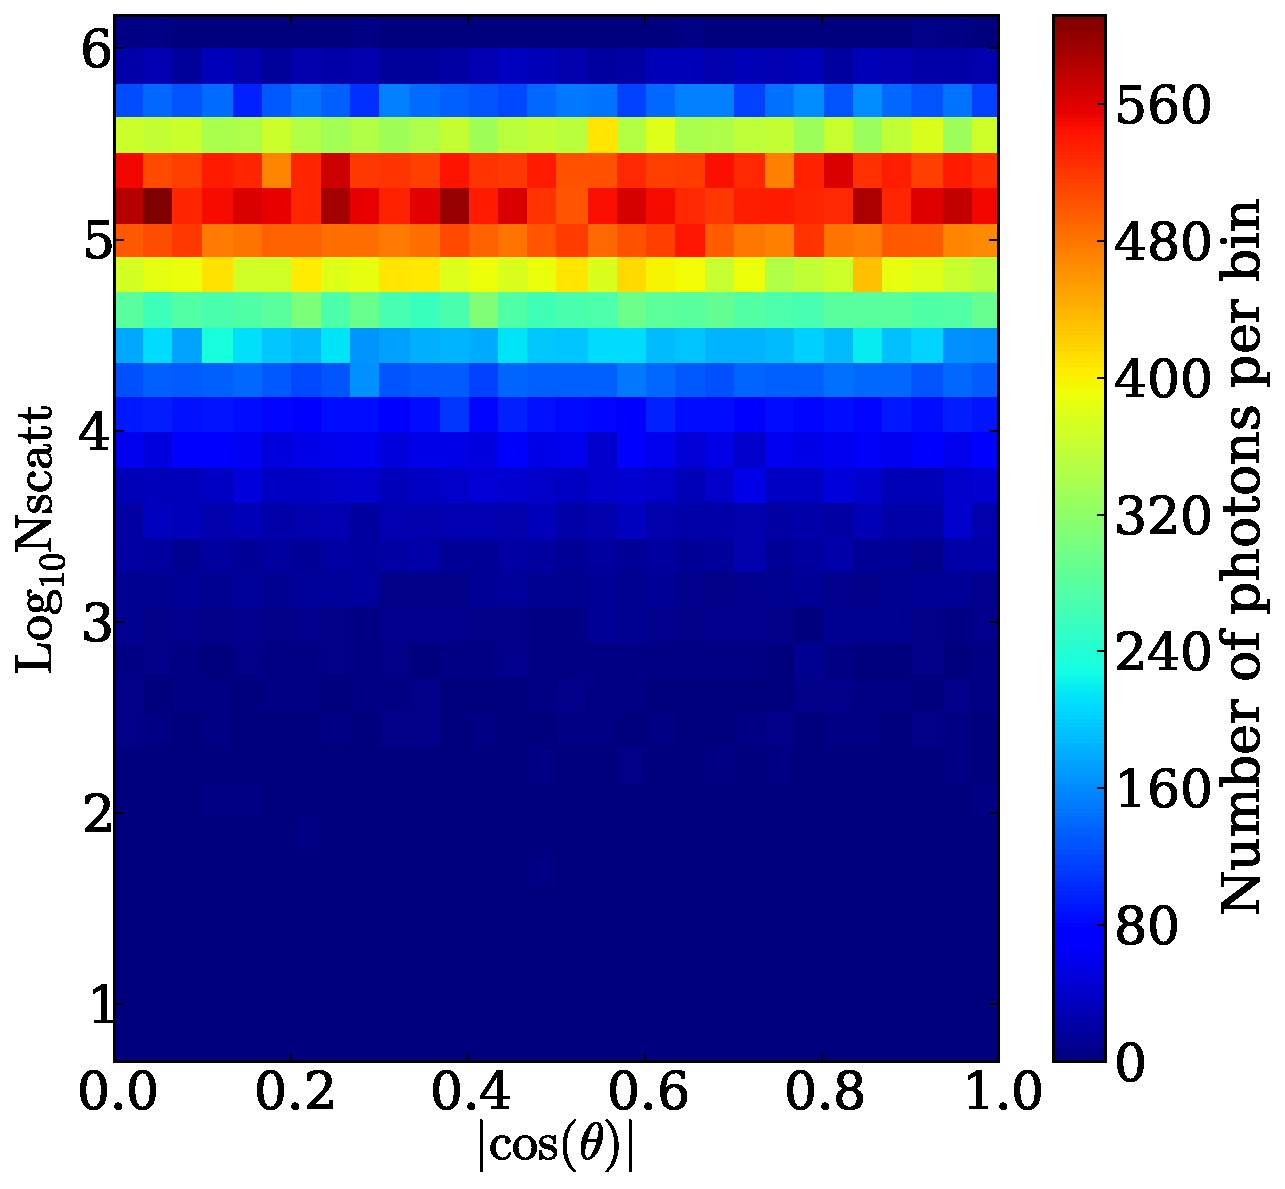
\includegraphics[width=0.45\textwidth]{../Figures/f12.pdf}
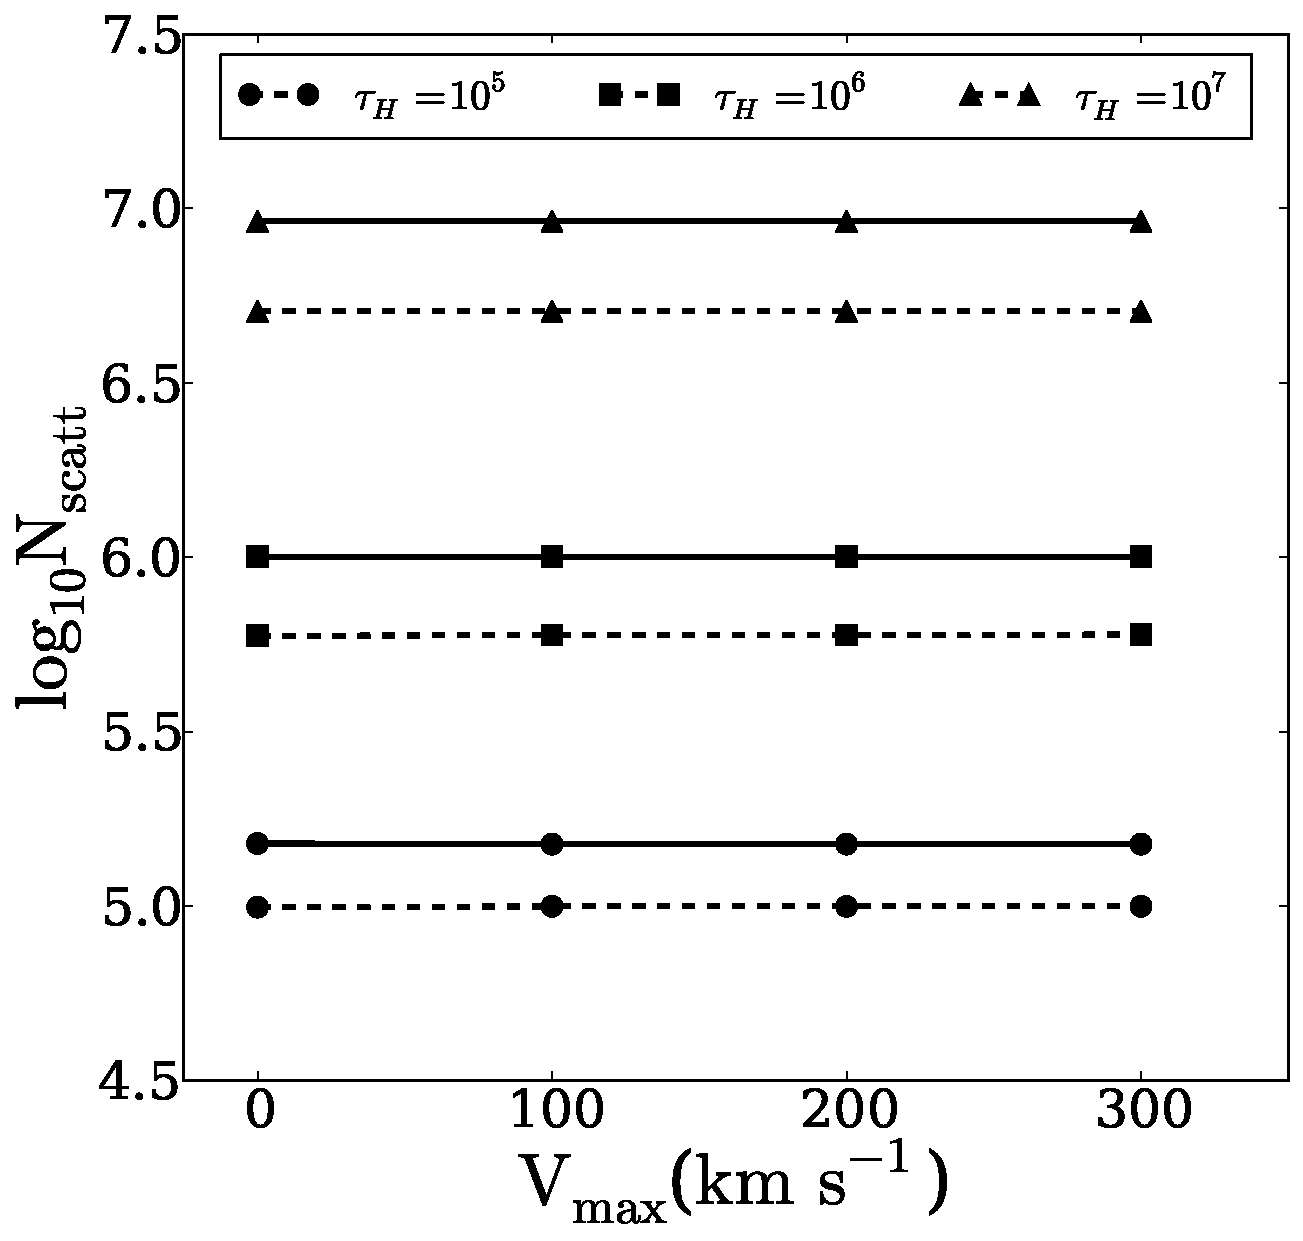
\includegraphics[width=0.45\textwidth]{../Figures/f13.pdf}
\end{center}
\caption{2D histogram of the logarithm of the average number of scatterings as function of $\mu$ (left) and the maximum rotational velocity $V_{\rm
max}$ (right). The left panel shows the behaviour for $\tau=10^{5}$ and
$V_{max}=300$\kms as a function of $\left|\cos\theta\right|$, the color indicates the number of photons per bin. In the
right panel the continous (dashed) lines represent the results for
the central (homogeneous) model. The independence of $N_{\rm scatt}$ with $\mu$ and $V_{\rm max}$ is
present in all models.
\label{fig:Nscatt} }
\end{figure*}
The number of scatterings affects the escape frequency of a \ly
photon. Studying this quantity further illustrates the independence of
the integrated flux and the escape fraction on rotational velocity.
In Fig. \ref{fig:Nscatt} we show the average number of scatterings
$\langle N_{\rm scatt}\rangle$ as a function of the cosinus of the
outgoing angle $|\cos\theta|$ and the rotational velocity
$V_{\rm max}$.
From the right panel observe that the number of scatterings and the
outgoing angle are independent.
This plot corresponds to the specific case of the central model with
$\tau=10^5$ and $V_{\rm max}=300$\kms, but we have verified that this
holds for all models.
The right panel of Fig. \ref{fig:Nscatt} shows how the average
number of scatterings is also independent from the rotational
velocity.
The lower number of average scatterings in the homogeneous source
distribution is due to a purely geometrical effect.
Photons emitted close to the surface go through less scatterings
before escaping.
In static configurations it is expected that the optical depth correlates number of
scatterings.
This has been precisely quantified in the case of static infinite
slab.
In that model for centrally emitted sources the average number of
scatterings depends only on the optical depth $\langle N_{\rm
scatt}\rangle=1.612\tau_{\rm H}$ \citep{Adams72,Harrington73}, for
homogeneously distributed sources $\langle N_{\rm
scatt}\rangle=1.16\tau_{\rm H}$ \citep{Harrington73}.
In our case we find that for the central model the number of
scatterings is proportional to the optical depth, with $\langle N_{\rm
scatt}\rangle= (1.50, 1.00, 0.92)\tau_{\rm H}$ for optical depth
values of $\tau_{\rm H} = (10^{5}, 10^{6}, 10^{7})$ respectively.
For the homogeneous sources we find that $\langle N_{\rm
scatt}\rangle= (0.99, 0.59, 0.51)\tau_{\rm H}$.

